\chapter{Scope and Problem Description}\label{scope and problem description}

This chapter discusses the Static E-scooter Battery Swap Rebalancing Problem (SEBSRP). Firstly in \Cref{problem scope}, the scope of the problem is presented, before a precise problem description is presented in \Cref{Problem Description}. Lastly an example of the problem is presented in \Cref{problem example}

\section{Scope}\label{problem scope}

 Consider an operator of an e-scooter company wanting to maximize the availability of its fleet by using their service vehicles. The main input for the operator is the locations of all e-scooters. Given this input, they want the optimal routes the service vehicles should take during a night shift. As the number of possible routes is numerous, and labor and service vehicle costs dominate, finding these optimal routes for maximizing the availability of the fleet will increase their operational profits. 

Minimizing the number of unavailable e-scooters will maximize the availability of the fleet. There are three possibilities for an e-scooter to be unavailable.
\begin{enumerate}
\item There is not enough battery on the e-scooter
\item The e-scooter is not near any customer
\item The e-scooter is broken and needs service before it can be used
\end{enumerate}

The operators solve these problems by:

\begin{enumerate}
\item Swapping batteries of e-scooters with a low battery level
\item Moving e-scooters from less attractive to more attractive zones
\item Picking up broken e-scooters for service
\end{enumerate}

Some terminology is now defined to make the reading easier. The action of changing the batteries of an e-scooter is referred to as a \textit{battery swap}. The action of picking up an e-scooter is named a \textit{pick-up} and the action of placing a picked-up e-scooter at a particular spot, a \textit{delivery}. The joint action of picking up and delivering an e-scooter is referred to as a \textit{rebalancing move}. 

This report does not consider picking up broken e-scooters for service. Hence, it will focus on battery swaps and rebalancing moves.

\Cref{fig:rebalancing_visualization} visualizes a rebalancing move where each location is represented as a circle. Above and beneath each location is the state before and after the rebalancing move. The service vehicle leaves the depot without any e-scooters. It then performs a pick-up at location 1, and delivery at location 2. The contribution to the objective function from this rebalancing move will be the avoidance of deviation from the optimal number of e-scooters at location 2.

\begin{figure}[H]
    \centering
    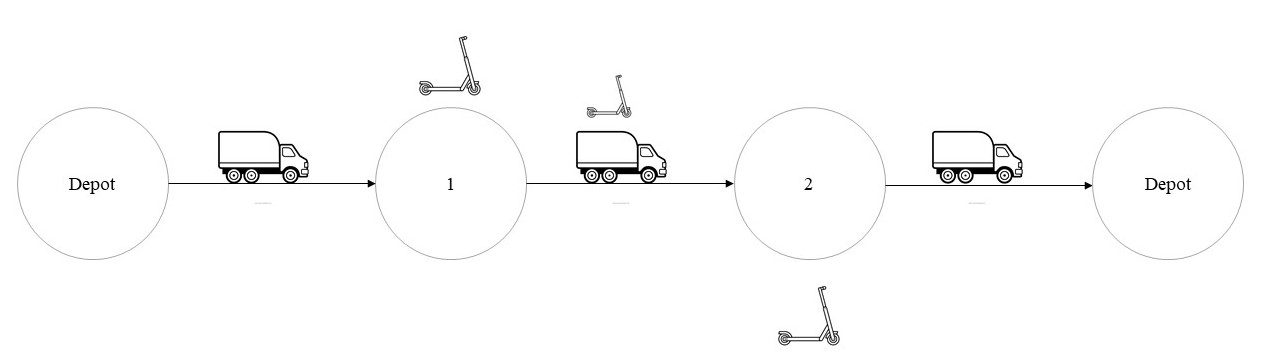
\includegraphics[width=0.8\textwidth]{Images/Visualisering av problem.jpg}
    \caption{Visualization of a rebalancing move}
    \label{fig:rebalancing_visualization}
\end{figure}

\section{Problem Description}\label{Problem Description}

The objective of the problem is to maximize the availability of the system. As the operators are not able to visit all e-scooters, they need to prioritize which e-scooters to visit. In order to do so, a reward is given for each e-scooter visited. This reward corresponds to the availability added by visiting a particular e-scooter. In this report, the reward is measured by the battery percentage added to the system. E.g. swapping the batteries of an e-scooter with a $70 \%$ battery level will add a reward of $0.3$. 

Additionally, the operator wants to rebalance its fleet. This means moving e-scooters from zones where there are too many e-scooters, to zones where there are too few. This is in order to ensure availability in zones with demand higher than the supply. To do so, the operator has defined geographical zones with corresponding ideal states. The ideal state of a zone is the ideal number of available fully charged e-scooters to exist in a zone after the rebalancing is done. When the operator receives the input data of the e-scooter positions, it knows what zones are demand and supply zones. The supply zones have more e-scooters than their ideal state, and the demand zones have less. The service vehicles can only pick up e-scooters in supply zones. A rebalancing move removes the availability in the zone where the e-scooter is picked up and adds availability in the zone where the e-scooter is delivered. The removed availability is equal to the battery percentage of the e-scooter, and the availability added to the delivery zone is equal to 1 as all rebalanced e-scooters receive a battery swap. 

The operator has defined some locations where e-scooters can be delivered. Hence, there are two types of locations, e-scooter- and delivery locations. As the operation is done at night, the e-scooters will not move during the operation. The time spent on each pick-up, delivery and battery swap is considered equal and is incorporated into the travel cost between the locations. Additionally, an action is performed at every location that is visited, implicating that some amount of time has to be assumed added at each location. The travel time is considered static, meaning that it will not change over time. Consequently, there is no consideration of rush traffic in this problem. The total time used for each service vehicle should not exceed the shift duration. Additionally, each service vehicle has an e-scooter capacity for pick-ups and a battery capacity for the number of battery swaps. The service vehicles have no e-scooters in their inventory when leaving or entering the depot and are not able to visit the depot to refill batteries during a shift.

All costs are treated as independent of how many battery swaps and rebalancing moves are done on a given route. This assumes that the service vehicles with staff are at work for the same number of hours every night with the same driving and wage cost. Hence, the cost is not part of the objective as it is constant for the same number of service vehicles and the same shift duration.

\section{Problem example}\label{problem example}

\Cref{fig:problem_example} shows a step by step example of a single route of a service vehicle in the problem. Each step represents a snapshot in time for the route. The gray ellipses represent zones and the arcs represent the sequential moves performed by the service vehicle. Batteries and e-scooters inside the car represent the inventory of the service vehicle. All of the e-scooters have an identification and a battery level associated with it. An opaque e-scooter in a zone represents a delivery location. The battery level is represented by a battery icon with different colors; green, yellow, and red indicating full, medium, and low battery levels. In this example the zone 1, 2, and 3 have an ideal state of 3, 1, and 2, respectively. Hence, zone 2 is a pick-up zone while zone 1 and 3 are delivery zones.

There are a few things to note about this example. The service vehicle is not able to perform a delivery in zone 1 as it does not have any e-scooters in its inventory when entering the zone. Additionally, when the service vehicle performs a pick-up in zone 2, it adds the e-scooter to its inventory. As all e-scooters picked up gets a battery swap, e-scooter 4 has a full battery when delivered to zone 3.

%Row 1
\begin{figure}[H]
    \centering
    \begin{subfigure}[H] {0.47\textwidth}
        \begin {tikzpicture}[-latex, auto, node distance =2cm and 2cm, on grid,
        depot/.style ={ rectangle,top color =white , bottom color = white ,
        draw,black, text=black , minimum size =0.5 cm}] \tikzmark{1}
            
            \node[opacity=0] (D)  {\includegraphics[scale=0.055]{Images/e-scooter_figures/car_1.PNG}};
            \node[] (C)  {\includegraphics[scale=0.055]{Images/e-scooter_figures/car_1.PNG}};
            \node[label={above:1}] (1) [above right =of C] {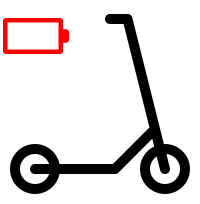
\includegraphics[scale=0.08]{Images/e-scooter_figures/e-scooter_0.png}};
            \node[label={below:2}] (2) [below right =of C] {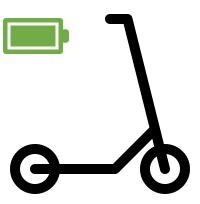
\includegraphics[scale=0.08]{Images/e-scooter_figures/e-scooter_100.png}};
            \node[label={above:3}] (3) [right =of 1] {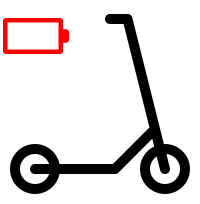
\includegraphics[scale=0.08]{Images/e-scooter_figures/e-scooter_0.png}};
            \node[label={below:4}] (4) [right =of 2] {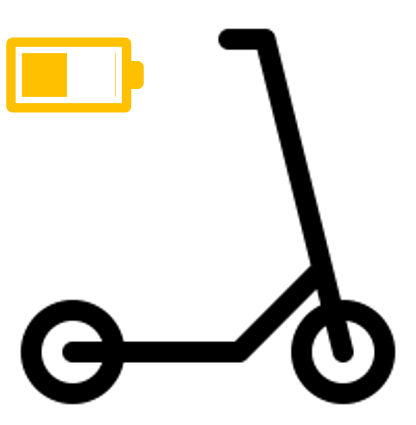
\includegraphics[scale=0.08]{Images/e-scooter_figures/e-scooter_50.png}};
            \node[label={below:5}] (5) [right = 5.5cm of C] {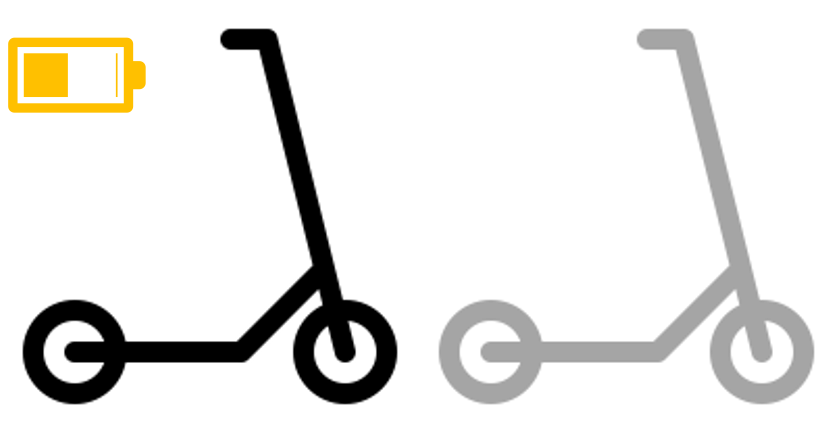
\includegraphics[scale=0.08]{Images/e-scooter_figures/e-scooter_50_D.png}};
            \node[] (DN) at (2.95, 2.7) {
\includegraphics[scale=0.08]{Images/e-scooter_figures/e-scooter_D.png}};
            \node[text width=3cm] at (4,1.2) {\small\textbf{Zone 1}};
            \node[text width=3cm] at (4,-1.2) {\small\textbf{Zone 2}};
            \node[text width=3cm] at (6.45,0.8) {\small\textbf{Zone 3}};

            \draw [fill=gray!10, opacity=0.2] (3,2) ellipse (2cm and 1.1cm);
            \draw [fill=gray!10, opacity=0.2] (3,-2) ellipse (2cm and 1.1cm);
            \draw [fill=gray!10, opacity=0.2] (5.5,0) ellipse (0.8cm and 1.5cm);
            
            \path (C) edge [] (1);
            \path (1) edge [] (3);
            \path (3) edge [] (4);
            \path (4) edge [] (5);
            
        \end{tikzpicture}
        \captionsetup[subfigure]{font={stretch=1.0}}
        \caption[Step 1]{Step 1 - The service vehicle leaves depot loaded with full batteries.}
        \label{fig:ex_1}
    \end{subfigure}
    \hspace*{5mm}
    \begin{subfigure}[H] {0.47\textwidth}
        \begin {tikzpicture}[-latex ,auto, , node distance =2cm and 2cm ,on grid,
        depot/.style ={ rectangle,top color =white , bottom color = white ,
        draw,black, text=black , minimum size =1 cm}] \tikzmark{2}
            
            \node[opacity=0] (D)  {\includegraphics[scale=0.055]{Images/e-scooter_figures/car_1.PNG}};
            \node[label={above:1}] (1) [above right = of D] {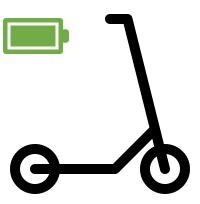
\includegraphics[scale=0.08]{Images/e-scooter_figures/e-scooter_100.png}};
            \node[] (C) [below = 15mm of 1] {\includegraphics[scale=0.055]{Images/e-scooter_figures/car_2.PNG}};
            \node[label={below:2}] (2) [below right =of D] {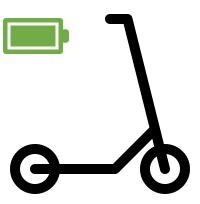
\includegraphics[scale=0.08]{Images/e-scooter_figures/e-scooter_100.png}};
            \node[label={above:3}] (3) [right =of 1] {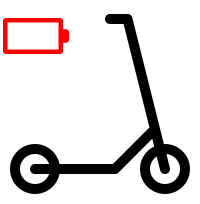
\includegraphics[scale=0.08]{Images/e-scooter_figures/e-scooter_0.png}};
            \node[label={below:4}] (4) [right =of 2] {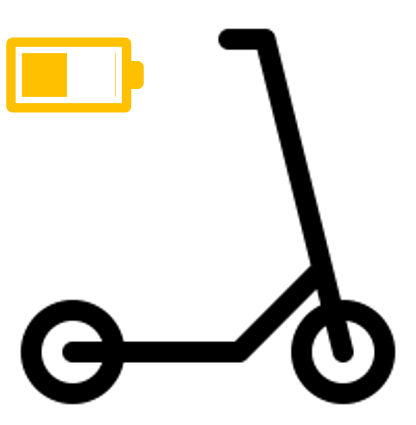
\includegraphics[scale=0.08]{Images/e-scooter_figures/e-scooter_50.png}};
            \node[label={below:5}] (5) [right = 5.5cm of D]
            {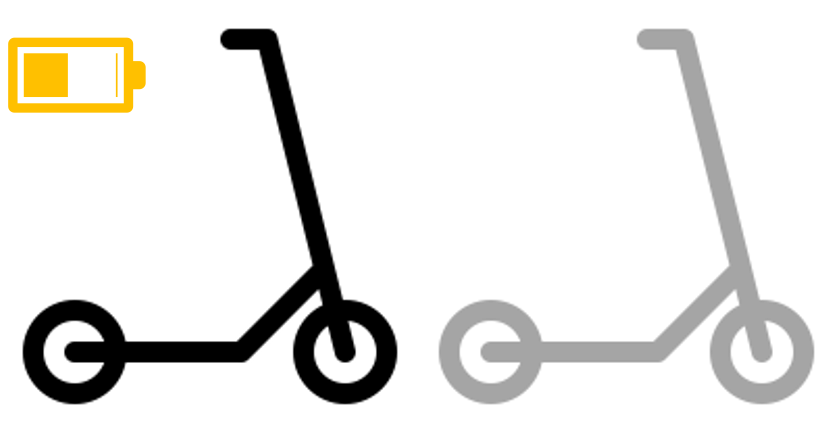
\includegraphics[scale=0.08]{Images/e-scooter_figures/e-scooter_50_D.png}};
            \node[] (DN) at (2.95, 2.7) {
\includegraphics[scale=0.08]{Images/e-scooter_figures/e-scooter_D.png}};
            \node[text width=3cm] at (4,1.2) {\small\textbf{Zone 1}};
            \node[text width=3cm] at (4,-1.2) {\small\textbf{Zone 2}};
            \node[text width=3cm] at (6.45,0.8) {\small\textbf{Zone 3}};

            \draw [fill=gray!10, opacity=0.2] (3,2) ellipse (2cm and 1.1cm);
            \draw [fill=gray!10, opacity=0.2] (3,-2) ellipse (2cm and 1.1cm);
            \draw [fill=gray!10, opacity=0.2] (5.5,0) ellipse (0.8cm and 1.5cm);
            
            \path (1) edge [] (3);
            \path (3) edge [] (4);
            \path (4) edge [] (5);

        \end{tikzpicture}
        \caption[Step 2]{Step 2 - The service vehicle arrives at the first e-scooter on the route and changes battery on e-scooter 1. }
        \label{fig:ex_2}
    \end{subfigure} 
    
    \bigskip

    \begin{subfigure}[H] {0.45\textwidth}
        \begin {tikzpicture}[-latex ,auto ,node distance =2cm and 2cm ,on grid ,
        depot/.style ={ rectangle,top color =white , bottom color = white ,
        draw,black, text=black , minimum size =0.5 cm}]
            
            \node[opacity=0] (D)  {\includegraphics[scale=0.055]{Images/e-scooter_figures/car_1.PNG}};
            \node[] (C) [below = 15mm of 3] {\includegraphics[scale=0.055]{Images/e-scooter_figures/car_3.PNG}};
            \node[label={above:1}] (1) [above right = of D] {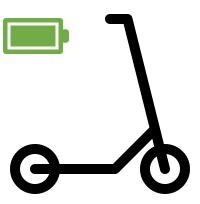
\includegraphics[scale=0.08]{Images/e-scooter_figures/e-scooter_100.png}};
            \node[label={below:2}] (2) [below right =of D] {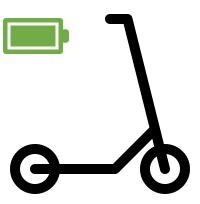
\includegraphics[scale=0.08]{Images/e-scooter_figures/e-scooter_100.png}};
            \node[label={above:3}] (3) [right =of 1] {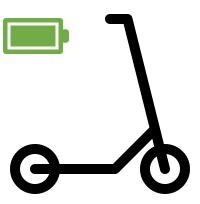
\includegraphics[scale=0.08]{Images/e-scooter_figures/e-scooter_100.png}};
            \node[label={below:4}] (4) [right =of 2] {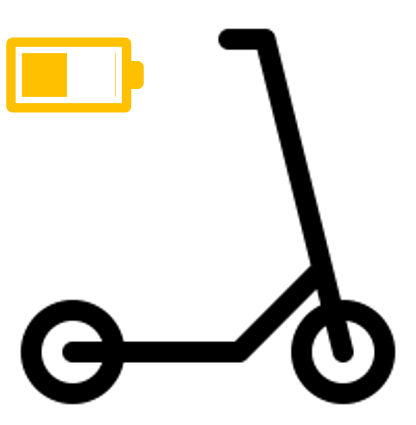
\includegraphics[scale=0.08]{Images/e-scooter_figures/e-scooter_50.png}};
            \node[label={below:5}] (5) [right = 5.5cm of D] {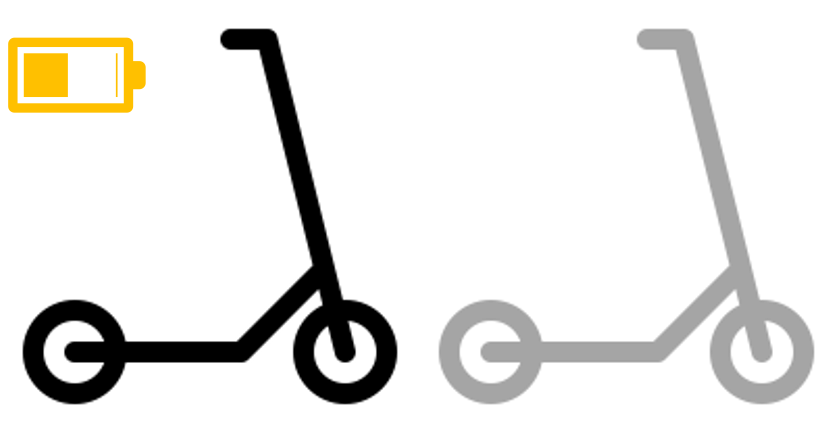
\includegraphics[scale=0.08]{Images/e-scooter_figures/e-scooter_50_D.png}};
            \node[] (DN) at (2.95, 2.7) {
\includegraphics[scale=0.08]{Images/e-scooter_figures/e-scooter_D.png}};
            \node[text width=3cm] at (4,1.2) {\small\textbf{Zone 1}};
            \node[text width=3cm] at (4,-1.2) {\small\textbf{Zone 2}};
            \node[text width=3cm] at (6.45,0.8) {\small\textbf{Zone 3}};

            \draw [fill=gray!10, opacity=0.2] (3,2) ellipse (2cm and 1.1cm);
            \draw [fill=gray!10, opacity=0.2] (3,-2) ellipse (2cm and 1.1cm);
            \draw [fill=gray!10, opacity=0.2] (5.5,0) ellipse (0.8cm and 1.5cm);
            
            \path (C) edge [] (4);
            \path (4) edge [] (5);
            
        \end{tikzpicture}
        \caption[Step 3]{Step 3 - The service vehicle arrives at the second e-scooter on the route and changes the battery on e-scooter 3.}
        \label{fig:ex_3}
    \end{subfigure} 
    \hspace*{10mm}
    \begin{subfigure}[H] {0.45\textwidth}
        \begin {tikzpicture}[-latex ,auto, , node distance =2cm and 2cm ,on grid,
        depot/.style ={ rectangle,top color =white , bottom color = white ,
        draw,black, text=black , minimum size =1 cm}]
            
            \node[opacity=0] (D)  {\includegraphics[scale=0.055]{Images/e-scooter_figures/car_1.PNG}};
            \node[] (C) [right = of 2] {\includegraphics[scale=0.05]{Images/e-scooter_figures/car_7.PNG}};
            \node[label={above:1}] (1) [above right = of D] {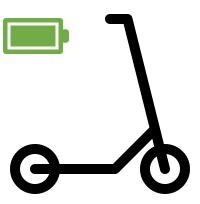
\includegraphics[scale=0.08]{Images/e-scooter_figures/e-scooter_100.png}};
            \node[label={below:2}] (2) [below right =of D] {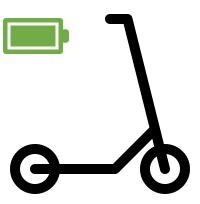
\includegraphics[scale=0.08]{Images/e-scooter_figures/e-scooter_100.png}};
            \node[label={above:3}] (3) [right =of 1] {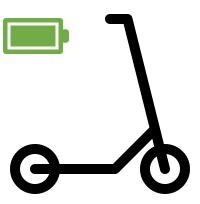
\includegraphics[scale=0.08]{Images/e-scooter_figures/e-scooter_100.png}};
            \node[label={below:5}] (5) [right = 5.5cm of D] {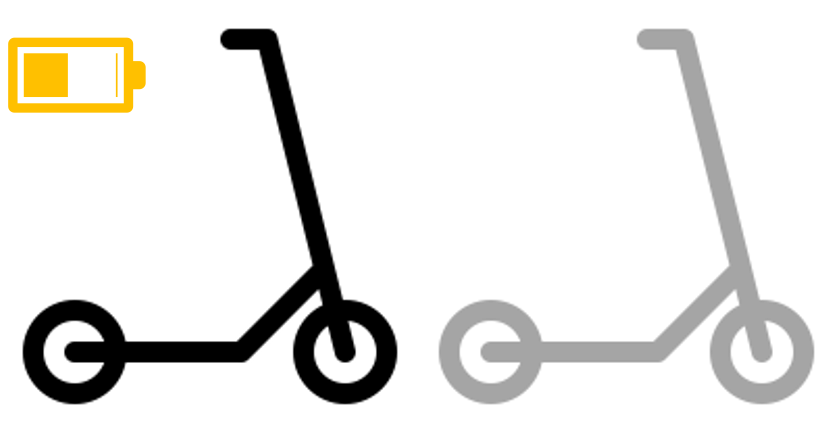
\includegraphics[scale=0.08]{Images/e-scooter_figures/e-scooter_50_D.png}};
            \node[] (DN) at (2.95, 2.7) {
\includegraphics[scale=0.08]{Images/e-scooter_figures/e-scooter_D.png}};
            \node[text width=3cm] at (4,1.2) {\small\textbf{Zone 1}};
            \node[text width=3cm] at (4,-1.2) {\small\textbf{Zone 2}};
            \node[text width=3cm] at (6.45,0.8) {\small\textbf{Zone 3}};

            \draw [fill=gray!10, opacity=0.2] (3,2) ellipse (2cm and 1.1cm);
            \draw [fill=gray!10, opacity=0.2] (3,-2) ellipse (2cm and 1.1cm);
            \draw [fill=gray!10, opacity=0.2] (5.5,0) ellipse (0.8cm and 1.5cm);
    
            \path (C) edge [] (5);
    
        \end{tikzpicture}
        \caption[Step 4]{Step 4 - The service vehicle arrives at the third e-scooter on the route and performs a pick up.}
        \label{fig:ex_4}
    \end{subfigure} \\
    
    \bigskip
    
    \begin{subfigure}[H] {0.45\textwidth}
        \begin {tikzpicture}[-latex ,auto ,node distance =2cm and 2cm ,on grid ,
        depot/.style ={ rectangle,top color =white , bottom color = white ,
        draw,black, text=black , minimum size =0.5 cm}]
            
            \node[opacity=0] (D)  {\includegraphics[scale=0.055]{Images/e-scooter_figures/car_1.PNG}};
            \node[] (C) at (5.65, -2) {\includegraphics[scale=0.05]{Images/e-scooter_figures/car_6.png}};
            \node[label={above:1}] (1) [above right =of D] {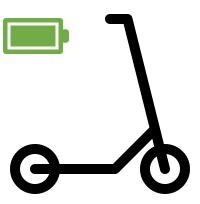
\includegraphics[scale=0.08]{Images/e-scooter_figures/e-scooter_100.png}};
            \node[label={below:2}] (2) [below right =of D] {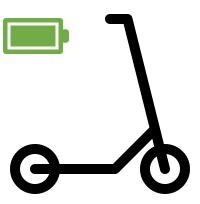
\includegraphics[scale=0.08]{Images/e-scooter_figures/e-scooter_100.png}};
            \node[label={above:3}] (3) [right =of 1] {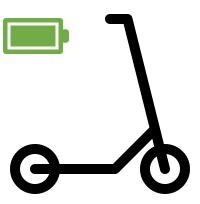
\includegraphics[scale=0.08]{Images/e-scooter_figures/e-scooter_100.png}};
            \node[label={below:5}] (5) [right = 5.5cm of D] {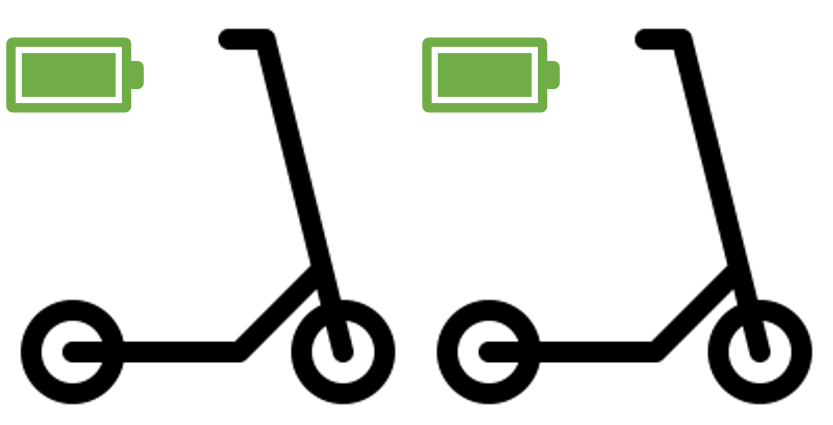
\includegraphics[scale=0.08]{Images/e-scooter_figures/e-scooter_100_2.png}};
            \node[] (DN) at (2.95, 2.7) {
\includegraphics[scale=0.08]{Images/e-scooter_figures/e-scooter_D.png}};
            \node[text width=3cm] at (4,1.2) {\small\textbf{Zone 1}};
            \node[text width=3cm] at (4,-1.2) {\small\textbf{Zone 2}};
            \node[text width=3cm] at (6.45,0.8) {\small\textbf{Zone 3}};

            \draw [fill=gray!10, opacity=0.2] (3,2) ellipse (2cm and 1.1cm);
            \draw [fill=gray!10, opacity=0.2] (3,-2) ellipse (2cm and 1.1cm);
            \draw [fill=gray!10, opacity=0.2] (5.5,0) ellipse (0.8cm and 1.5cm);
            
        \end{tikzpicture}
        \caption[Step 5]{Step 5 - The service vehicle arrives at the final e-scooter on the route, performs a battery swap and deliver e-scooter 4 at the delivery location.}
        \label{fig:ex_5}
    \end{subfigure} 
    \hspace*{10mm}
    \begin{subfigure}[H] {0.45\textwidth}
        \begin {tikzpicture}[-latex ,auto ,node distance =2cm and 2cm ,on grid ,
        depot/.style ={ rectangle,top color =white , bottom color = white ,
        draw,black, text=black , minimum size =0.5 cm}]
            
            \node[] (D) {\includegraphics[scale=0.05]{Images/e-scooter_figures/car_6.png}};
            \node[label={above:1}] (1) [above right =of D] {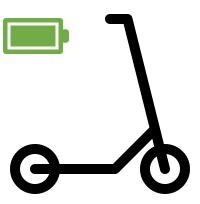
\includegraphics[scale=0.08]{Images/e-scooter_figures/e-scooter_100.png}};
            \node[label={below:2}] (2) [below right =of D] {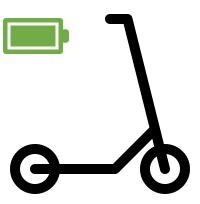
\includegraphics[scale=0.08]{Images/e-scooter_figures/e-scooter_100.png}};
            \node[label={above:3}] (3) [right =of 1] {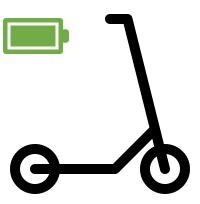
\includegraphics[scale=0.08]{Images/e-scooter_figures/e-scooter_100.png}};
            \node[label={below:5}] (5) [right = 5.5cm of D] {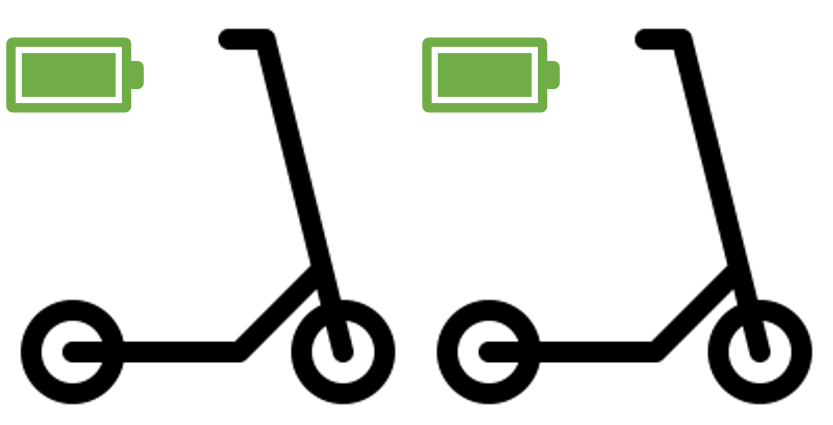
\includegraphics[scale=0.08]{Images/e-scooter_figures/e-scooter_100_2.png}};
            \node[] (DN) at (2.95, 2.7) {
\includegraphics[scale=0.08]{Images/e-scooter_figures/e-scooter_D.png}};
            \node[text width=3cm] at (4,1.2) {\small\textbf{Zone 1}};
            \node[text width=3cm] at (4,-1.2) {\small\textbf{Zone 2}};
            \node[text width=3cm] at (6.45,0.8) {\small\textbf{Zone 3}};

            \draw [fill=gray!10, opacity=0.2] (3,2) ellipse (2cm and 1.1cm);
            \draw [fill=gray!10, opacity=0.2] (3,-2) ellipse (2cm and 1.1cm);
            \draw [fill=gray!10, opacity=0.2] (5.5,0) ellipse (0.8cm and 1.5cm);
            
        \end{tikzpicture}
        \caption[Step 6]{Step 6 - Service vehicle returns to the depot and all zones are in ideal state.}
        \label{fig:ex_6}
    \end{subfigure} 
    \caption{Step by step problem example}
    \label{fig:problem_example}
\end{figure}




